\section{Métodos}
En este trabajo se ha llevado a cabo una revisión sistemática de la literatura científica publicada en materia de ciencias de la computación en relación con metodologías en ciencia de datos para el diagnostico del cáncer de mama. Para su elaboración, se han seguido las directrices de la declaración PRISMA \citep{Moher2009} para la correcta realización de revisiones sistemáticas. A continuación se detallan las etapas realizadas en el proceso.
\begin{figure}[h!]
	\centering
	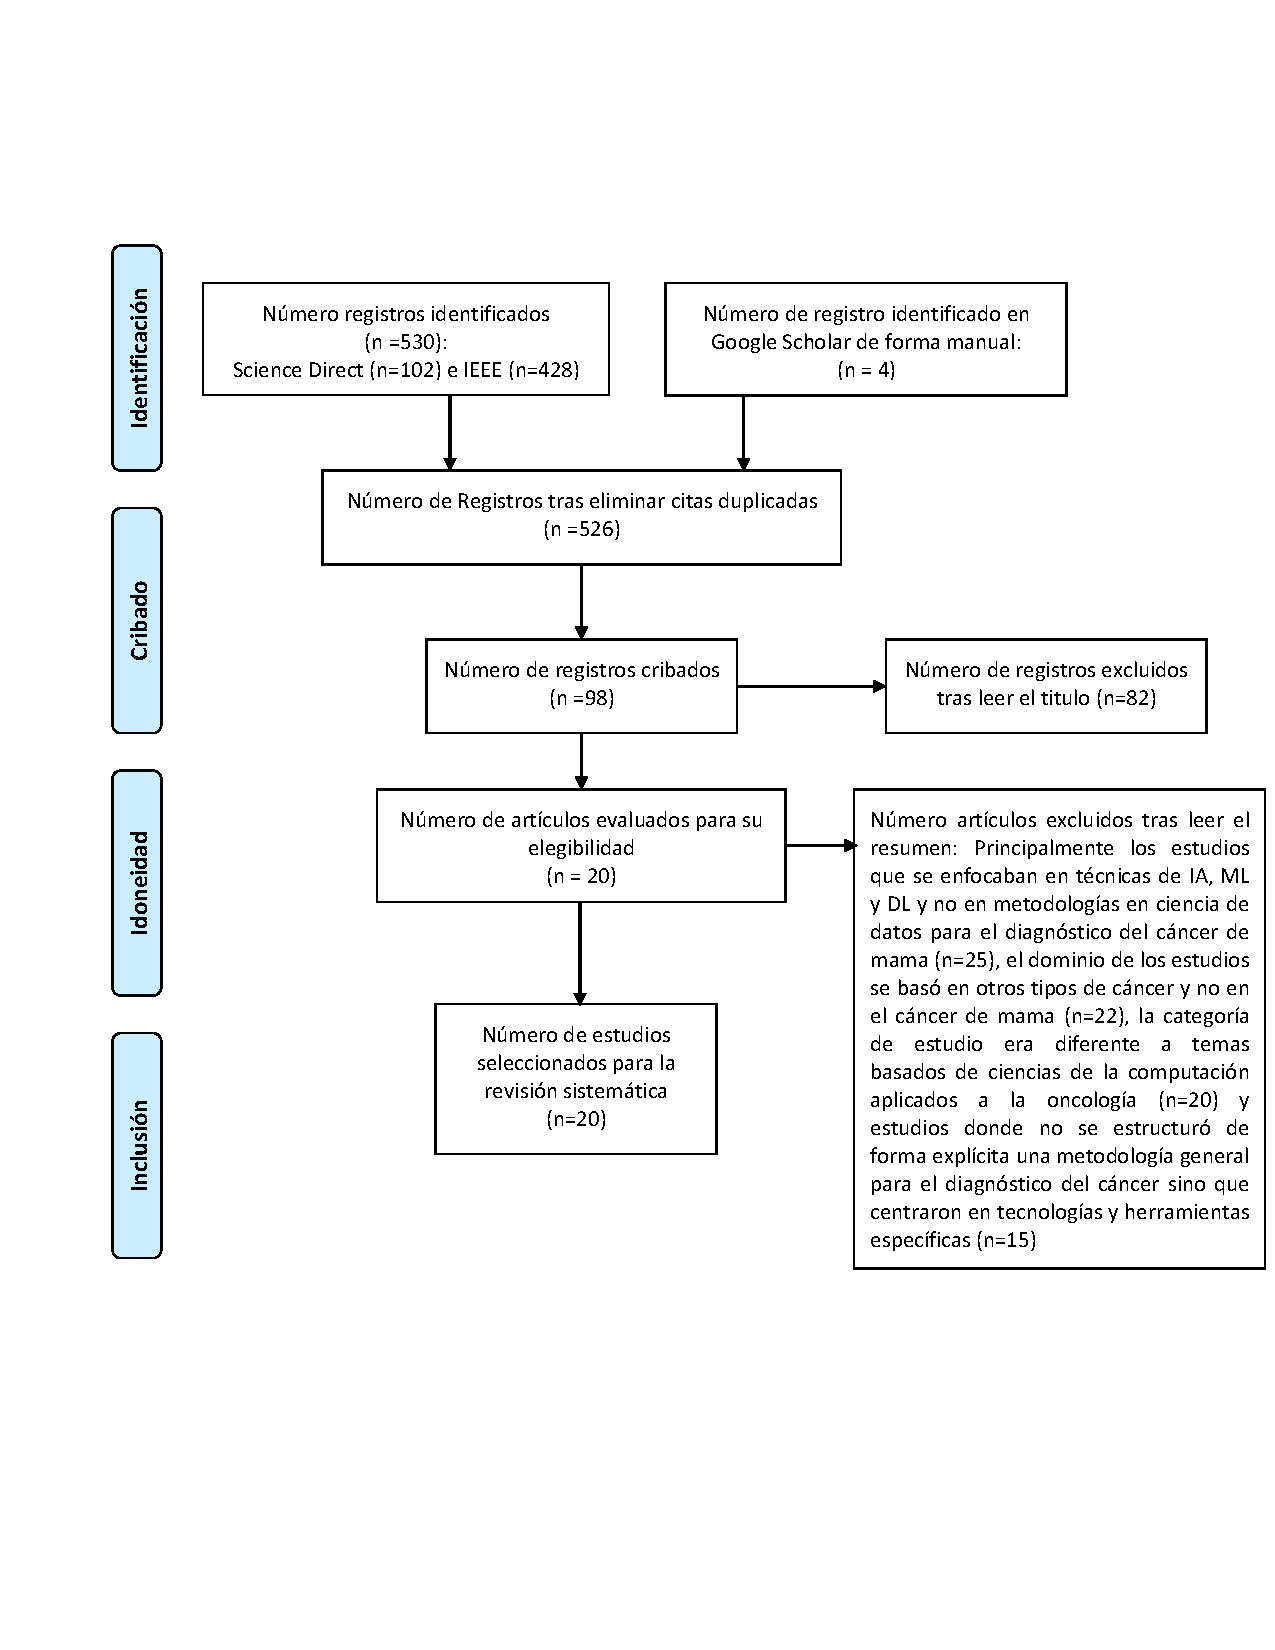
\includegraphics[width=1
	\linewidth]{IMAGENES/PRISMA_DIAGRAM}
	\caption{Diagrama de flujo PRISMA en cuatro niveles }
	\label{Diagrama_Prisma}
\end{figure}

\subsection{Búsqueda inicial}
Las primeras búsquedas se realizaron en abril de 2021 combinando los términos \textit{data science, breast cancer, deep learning, machine Learning, artificial intelligence, cancer Biopsy ,Core needle biopsy, Fine needle aspiration} en las bases de datos de IEEE Access, Nature Reviews Cancer, Elsevier y Science Direct. Posteriormente, para generar una búsqueda mas especifica acerca de metodologías en ciencia de datos aplicadas al diagnostico del cáncer de mama se realizó la combinación de estos términos usando los operadores booleanos \textit{AND} y \textit{OR}. Los resultados obtenidos en la búsqueda arrojaron una cantidad excesiva de literatura basada en técnicas de Inteligencia Artificial, Machine Learning y Deep Learning aplicadas al diagnostico de esta enfermedad sin tener una metodología clara en ciencia de datos aplicada a esta área de la salud, por lo cual dichos resultados fueron poco útiles para la revisión. Sin embargo, las consultas realizadas permitieron tener un visión global de la complejidad del tema de investigación y los diferentes enfoques que pueden generarse a nivel de ciencia de la computación si no se limita la temática al rededor de una metodología.

Debido a que los resultados arrojados por Nature Reviews Cancer y The Lancet estaban enfocados en técnicas y no metodologías, lo cual no aportada información relevante al estudio, se decidió su eliminación de la búsqueda sistemática.  

\subsection{Búsqueda sistemática}
La búsqueda sistemática se realizo en febrero del 2022, en IEEE Access y Science Direct, acotando los resultados de publicaciones realizadas en 2014 hasta la actualidad. La combinación de términos que arrojó mejores resultados en ambos buscadores fue la siguiente:
\textit{(methodology AND Data Science) OR (methodology AND diagnose AND cancer) OR (data science AND methodology AND health AND diagnostics) OR (data science AND methodology AND breast AND cancer)}.

Concretamente, se obtuvieron $530$ resultados de los cuales $428$ fueron encontrados en IEEE Access y $102$ en Science Direct. Antes de realizar la selección de artículos, se definieron los siguientes criterios de inclusión y exclusión. 

\begin{itemize}
	
	\item{\textbf{\textit{Criterios de inclusión}}}
	\begin{itemize}
		\item Tratarse de artículos de investigación, revisión sistemática, libros o manuales. 
		\item Que los estudios realizados estén basadas en metodologías en ciencia de datos  y no en técnicas de Inteligencia Artificial, Machine Learning y Deep Learning.
		\item Que la categoría de estudio este bajo la temática de ciencias de la computación aplicado a la oncología.
		\item Que el dominio determinado este enfocado en el diagnostico del cáncer de mama.
		\item Que los articulo de investigación realizados no dependan de tecnologías ni herramientas específicas.
		\item Que se hayan publicado entre 2014 y 2022, ambos inclusive.
		
	\end{itemize}
	
	\item{\textbf{\textit{Criterios de exclusión}}}
	\begin{itemize}
		\item Se excluyen los estudios que se enfoquen en técnicas de Inteligencia Artificial, Machine Learning y Deep Learning y no en metodologías en ciencia de datos. 
		\item Estudios en donde el dominio se base en otros tipos de cáncer y no en el cáncer de mama.
		\item Estudios donde la categoría sea diferente a temas basados de ciencias de la computación aplicados a la oncología. 
		\item Estudios donde no se evidencie de forma explícita una estrategia general para el diagnóstico del cáncer sino se centren en otros temas, tecnologías y herramientas específicas.
	\end{itemize}
	
\end{itemize}

Según estos criterios, y sólo con la lectura del titulo se consideraron adecuados $98$ artículos. Posteriormente, se realizo la lectura del resumen y a partir de esta lectura, se descartaron $82$ artículos, principalmente los estudios que se enfocaban en técnicas de Inteligencia Artificial, Machine Learning y Deep Learning y no en metodologías en ciencia de datos para el diagnóstico del cáncer de mama ($n=25$), el dominio de los estudios se basó en otros tipos de cáncer y no en el cáncer de mama ($n=22$), la categoría de estudio era diferente a temas basados de ciencias de la computación aplicados a la oncología ($n=20$) y estudios donde no se estructuró de forma explícita una metodología general para el diagnóstico del cáncer sino que centraron en tecnologías y herramientas específicas ($n=15$). Finalmente, $16$ artículos encontrados en IEEE Access y Science Direct cumplieron con los criterios de inclusión y se seleccionaron para llevar a cabo la revisión sistemática. 

\subsection{Búsqueda Manual}
Al realizar una lectura detallada de las $16$ investigaciones encontradas en la búsqueda sistemática, basándonos en sus referencias para comprobar si existía información adicional relacionada con el tema de estudio, se empleo Google Scholar con los términos de búsqueda descritos anteriormente y como resultado se incluyeron $3$ capítulos de libros de ciencias de la computación que abarcaban diferentes metodologías en ciencia de datos y $1$ articulo de investigación encontrado en la revista IJSR\footnote{International Journal of Science and Research } que contenía información relevante para la investigación. 

En definitiva, $20$ investigaciones entre artículos y capítulos de libros publicados entre 2014 y 2022 fueron seleccionados para realizar la revisión sistemática de la aplicación de la ciencia de datos en metodologías para el diagnóstico del cáncer de mama (Figura \ref{Diagrama_Prisma}).